\documentclass[tikz]{standalone}
\usepackage{pgfplots}
\pgfplotsset{compat=1.15}
\usepackage{mathrsfs}
\usetikzlibrary{arrows,calc}
\usepackage{tkz-euclide}
\pagestyle{empty}

\definecolor{AngleClr}{rgb}{0,0.39215686274509803,0}
\definecolor{ShapeClr}{rgb}{0.6,0.2,0}

\begin{document}

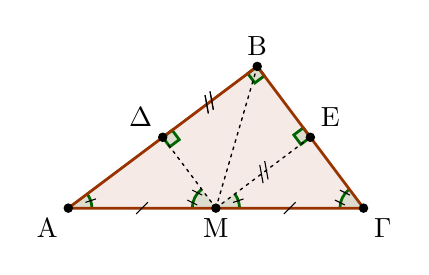
\begin{tikzpicture}[scale=.75]
\tkzSetUpLine[line width=1pt,color=black]
\tkzSetUpPoint[fill=black]

\tkzDefPoints{0/0/A,3.2/2.4/B,5/0/C,2.5/0/O}

\tkzDefPointBy[projection=onto B--A](O)\tkzGetPoint{D}
\tkzDefPointBy[projection=onto B--C](O)\tkzGetPoint{E}

\tkzFillPolygon[fill=ShapeClr,fill opacity=0.1](A,B,C)
\tkzFillAngles[fill=AngleClr,size=.4,fill opacity=0.1](C,A,B C,O,E B,C,A D,O,A)
\tkzMarkAngles[mark=|,mksize=2,line width=1pt,size=.4,color=AngleClr](C,A,B C,O,E)
\tkzMarkAngles[mark=||,mksize=2,line width=1pt,size=.4,color=AngleClr](B,C,A D,O,A)

\tkzMarkRightAngles[line width=1pt, size=.2,color=AngleClr,fill=AngleClr,fill opacity=0.1](A,B,C O,D,B O,E,B)

\tkzDrawSegments[line width=0.5pt,color=black,dashed,dash pattern=on 1pt off 1.75pt](O,B O,D O,E)

\tkzDrawPolygon[color=ShapeClr](A,B,C)
\tkzDrawPoints[size=3](A,B,C,D,E,O)
\tkzLabelPoint[below left](A){$\mathrm{A}$}
\tkzLabelPoint[above](B){$\mathrm{B}$}
\tkzLabelPoint[below right](C){$\mathrm{\Gamma}$}
\tkzLabelPoint[below](O){$\mathrm{M}$}
\tkzLabelPoint[above left](D){$\mathrm{\Delta}$}
\tkzLabelPoint[above right](E){$\mathrm{E}$}

\tkzMarkSegments[mark=s|,size=3](O,A O,C)
\tkzMarkSegments[mark=s||,size=3](O,E B,D B,D)


\end{tikzpicture}

\end{document}
